\part{The Aircraft}
\chapter{General Description}

\chapter{Systems}

\section{Auxiliary Power Unit (APU)}
\label{sec:apu}

A Honeywell Aerospace GTCP85-180L \gls{APU} is located in the forward part of the left wheel well. The \gls{APU} is a small, self-contained, single shaft gas turbine operating at a constant speed of approximately 42.000 \gls{RPM}. A shaft driven 40 \gls{kVA} AC generator supplies power to the electrical system. During ground operation bleed air can be used for engine starting and operation of the air-conditioning systems. Using the aircraft battery to start the \gls{APU} allows for operations on remote locations, without any ground support equipment available.

%Electrical starter, control circuits and ignition are powered through the Isolated DC bus.

\subsection{Fuel System}

The APU uses the same fuel as used for the main engines. Depending on the applied load, typical fuel consumption varies between 130 \gls{lbs/hr} and 270 \gls{lbs/hr}.

\paragraph*{Fuel Supply}
Fuel is gravity feed from the No. 2 main tank through a firewall shutoff valve installed in the No. 2 dry bay. The shutoff valve prevents fuel flow anytime the \gls{APU} control switch is placed in the STOP position, the \gls{APU} fire handle is pulled or the \gls{APU} control circuits are deengerized.

\paragraph*{Fuel Control Unit}
The fuel control unit fully automatically operates the fuel pump. Using a shaft governor the amount of fuel supplied to the combustor is varied to keep the rotational speed constant. A thermostat limits the fuel flow to protect the turbine from overtemperature, effectively also limiting acceleration during starting. While extracting bleed air, temperature limiting is shifted to the \nameref{par:bleed-air-shutoff-and-load-control-valve}.

\paragraph*{Fuel Shutoff Valve}
\label{par:fuel-shutoff-valve}
At the outlet of the fuel control unit another fuel shutoff valve opens once reaching a minimum oil pressure. During startup it opens at approximately 10\% \gls{RPM}. If oil pressure is lost the valve closes and the \gls{APU} will automatically shut down.

\subsection{Oil System}

A pressurized oil system provides lubrication to gears and shaft bearings. The shaft driven oil pump delivers oil from an external reservoir to the gears and bearings. A relieve valve maintains an operating pressure within 90$\pm$10 \gls{psi} while the \gls{APU} operates at 100\% \gls{RPM}. Oil temperature is regulated by either directing oil flow through the oil cooler, or if oil temperature is below 27°C, through the oil cooler by-pass valve.

\paragraph*{Oil-pressure sequencing switch}
At approximately 15\% \gls{RPM} oil pressure is sufficient to operate the oil-pressure sequencing switch, which completes circuits to the \nameref{par:fuel-shutoff-valve} and ignition system. It prevents starting without lubrication and ensures an adequate airflow for combustion before introducing fuel and initiating ignition.

\paragraph*{Door-control oil-pressure switch}
Oil pressure below 20 \gls{psi} (equals approximately 18\% \gls{RPM}) operates the door-control oil-pressure switch allowing to close the \nameref{par:air-intake-door}. This is done to prevent collapse of the air inlet duct due to build-up of negative pressure.

%\begin{bclogo}[logo=\bclampe, ombre=true, couleurOmbre = black!80, couleurBarre=blue, marge=6]{Note}
\begin{bclogo}[logo=\bclampe, ombre=false, couleurBarre=blue, marge=18, noborder=true]{Note}
\indent
Placing the APU control switch in the "STOP" position or pulling the APU fire handle is required to complete the circuit for actually closing the \nameref{par:air-intake-door}.
\end{bclogo}

\subsection{Airflow}

\paragraph*{Air Intake Door}
\label{par:air-intake-door}

\paragraph*{Bleed Air Shutoff and Load Control Valve}
\label{par:bleed-air-shutoff-and-load-control-valve}

\subsection{Controls and Indications}

\nameref{sec:apu-panel} and \nameref{sec:bleed-air-panel}

%40 KVA AC generator, electrical power up to 20.000 feet.

%APU air inlet door closes if APU control switch is in STOP position and oilpressure decreases below approximately 20 PSI, which happens at about 18 percent \gls{RPM}.

%Starter approx. 1100 Watt. inrush current 4-8 times normal

APU bleed air valve switch on the Bleed Air Panel.

\section{Advisory, Caution and Warning System (ACAWS)}
\label{sec:acaws}

\gls{ACAWS}

\section{Electric System}

2 batteries: Utility, Avionics 24V 42Ah at C1

\#2 generator powers essential AC bus, if \#2 lost APU powers essential AC bus (APU always powers essential AC bus if online), else \#1 takes load (same side takes/assumes load). If two engines/generators on same side shutdown/lost, symmetrical engines pick up loads.

\#1 generator: Left Hand AC bus.\\
\#2 generator powers Essential AC bus.\\
\#3 generator will power the Main AC bus.\\
\#4 generator will power the Right Hand AC bus.

Gen 1-4 and APU ACAWS Indications. When the GCU detects an out of tolerance condition, and a generator switch or EXT PWR/OFF/APU switch is in ON (generator) or APU (apu), it will open the line contactor and send a system status indication to the bus interface unit BIU. The
BIU will then generate a data word to the mission computer that a failure has occurred in one of the engine generators or the APU generator. An advisory, caution, and warning system (ACAWS) text message (GEN 1,2,3, or 4 FAIL or APU GEN FAIL) will then be displayed for the first ten
seconds in reverse color (black letters on a night vision imaging system (NVIS) yellow background) followed by flashing master caution lights.

\section{Avionics System}

The \gls{BIU}s convert various signals and serve as additional backup bus controllers (and somehow the Mission Computers?).

\section{Hydraulic System}

Utility hydraulic system: wing flaps, main landing gear, normal braking, nose wheel steering.

\section{Enhanced Cargo Handling System (ECHS)}
\label{sec:echs}

\gls{MFCD}, \gls{RECP}, \gls{CAWS} 12 pairs of electric pallet locks (40 inch spacing) http://www.google.com/patents/EP0771726A2?cl=en

\subsection{Cargo Compartements}

\begin{itemize}
  \itembf{C} 245 - 281
  \itembf{D} 281 - 337
  \itembf{E} 337 - 401
  \itembf{F} 401 - 457
  \itembf{G} 457 - 517
  \itembf{H} 517 - 597
  \itembf{I} 597 - 627
  \itembf{J} 627 - 682
  \itembf{K} 682 - 737
  \itembf{L} 737 - 803 (Ramp)
  \itembf{M} 803 - 869 (Ramp)
\end{itemize}

\subsection{Locks}

\begin{enumerate}
  \item 302
  \item 342
  \item 382
  \item 422
  \item 462
  \item 502
  \item 542
  \item 582
  \item 622
  \item 662
  \item 682
  \item 803?
\end{enumerate}

% right 884px/885px
% left 80px/87px
% total 800px -> l: 112px, r: 912

\chapter{Cockpit Controls}

Blah blah

\section{Overhead Panel}

\subsection{Electrical Panel}

\begin{enumerate}
  \itembf{Battery (BTRY) switch} Connects battery bus to isolated DC bus.
\end{enumerate}

\subsection{Bleed Air Panel}
\label{sec:bleed-air-panel}

\begin{enumerate}
  \itembf{\gls{APU} Bleed Air Valve switch}{OPEN/CLSD}
  \itembf{Divider Valve switch}{CLOSE/AUTO/OPEN}
  \itembf{Wing Isolation Valve switches}{CLOSE/AUTO/OPEN}
  \itembf{Nacelle Shutoff Valve switches}{CLOSE/AUTO/OPEN}
\end{enumerate}

\subsection{Fuel Management Panel}

Transfer switches (TO/FROM)

\subsection{Engine Start and Fire Control Panel}
\label{sec:eng-panel}

\begin{enumerate}
  \itembf{Engine 1/2/3/4 Fire Handle}
  \itembf{Engine 1/2/3/4 Start switch}
    \begin{itemize}
      \itembf{MOTOR}
      \itembf{STOP}
      \itembf{RUN}
      \itembf{START}
    \end{itemize}
    Fuel pumps in respective tank operated in RUN/START and stopped in MOTOR/STOP
\end{enumerate}

\subsection{APU Panel}
\label{sec:apu-panel}

The \gls{APU}...

\begin{enumerate}
  \itembf{Control switch}
    \begin{itemize}
      \itembf{STOP} Same as 110\% overspeed switch. APU door closes if below 18\% (or oilpressure below 20 PSIG).
      \itembf{RUN} APU door opens.
      \itembf{START}{spring-loaded position} If APU door opened at least 15° starter engages
    \end{itemize}
  \itembf{\gls{EGT} indication}
  \itembf{\gls{RPM} indication}
  \itembf{Fire handle} The T-shaped fire handle
    \begin{enumerate}
      \item Control power interrupt
      \item Fuel shut-off valve closes
      \item Once the APU \gls{RPM} falls below approximately 18\% the APU air intake door is closed.
      \item Agent discharge switching available
    \end{enumerate}
\end{enumerate}

\section{Instrument Panel}

\subsection{Avionics Management Unit (AMU)}
\label{sec:amu}

The \gls{AMU}, \gls{CNBP}, \gls{CMDU}, \gls{CMDS}

\subsection{Head Down Displays (HDD)}
\label{sec:hdd}

Readouts are color coded. Information will be presented in white when in the normal operating range, yellow for information out of the normal range but not out of limits, and red for out of limit values.

\newpage
\subsubsection{Primary Flight Display (PFD)}
\label{sec:pfd}

The \gls{PFD}...

%\newpage
\subsubsection{Engine}

\newpage
\subsubsection{System Status}

The SYSTEM STATUS display consists of multiple sections:

\begin{figure}[h]
  \centering
  \colorbox{black}{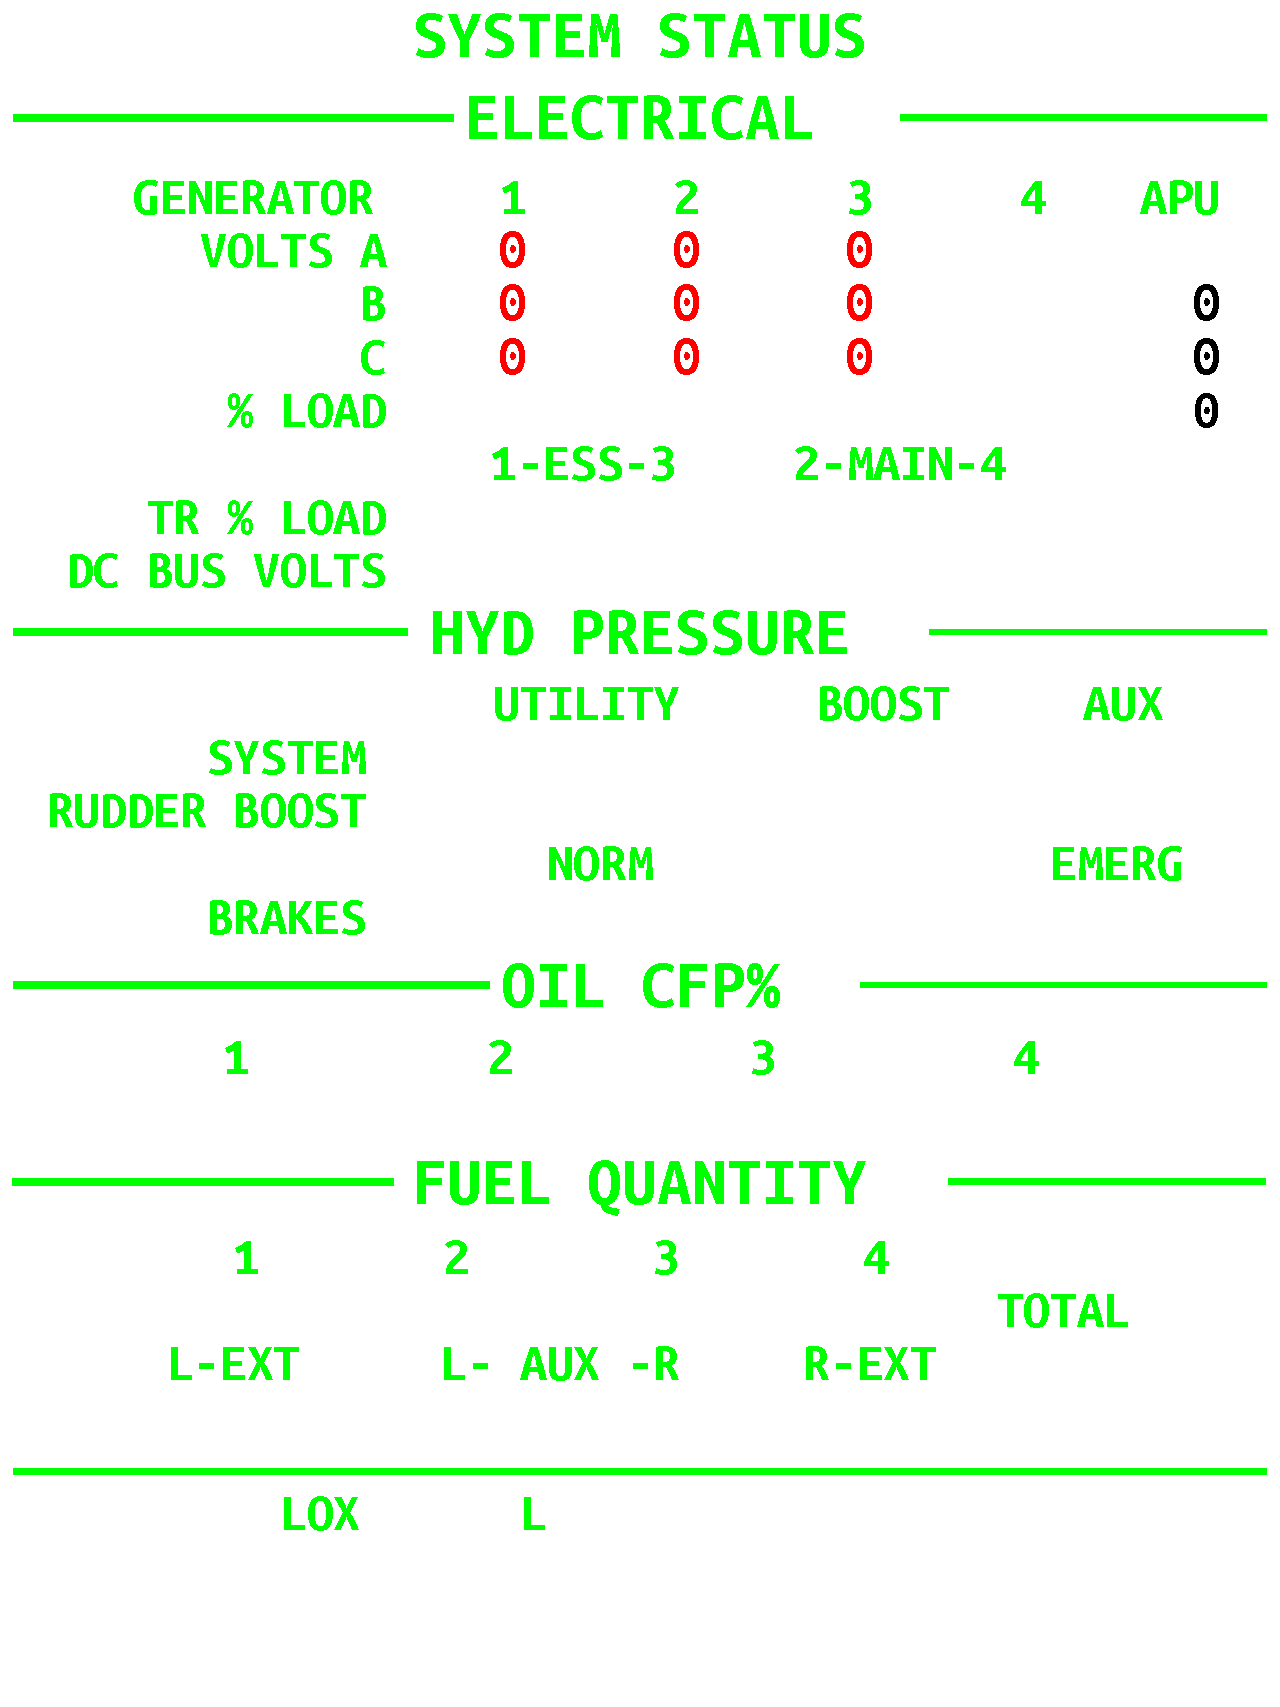
\includegraphics[width=7cm]{figures/hdd/SYSTEM-STATUS}}
  \caption{SYSTEM STATUS display}
\end{figure}

\paragraph*{ELECTRICAL}
Generator voltage and percentage of rated current load are shown. Values for generator voltage and load are displayed in columns, labeled from left to right, representing generators 1, 2, 3, 4 and the APU generator. Three voltages are shown in the column for each generator to indicate the voltage of each of the three phases of the generator: A phase, B phase, C phase. Percent of maximum rated load for all five generators (an average of the three phases) is displayed in the row below the C phase voltage. If the system is not powered, OFF will be displayed in the appropriate data blocks. If the system is disconnected (eg. EXT PWR/OFF/APU not APU for APU), three dashed lines will be displayed. The display symbols are generated by the multifunction display units based on information received from the mission computer. 

\paragraph*{HYD PRESSURE}

\paragraph*{OIL CFP\%}

\paragraph*{FUEL QUANTITY}

\subsection{Autopilot}

Reference Settings
\begin{enumerate}
  \itembf{HP}
  \itembf{RAD ALT} Radar altitude
  \itembf{IAS} \gls{IAS}
  \itembf{FPA} \gls{FPA}
  \itembf{MINS}
\end{enumerate}

Mode Selections
\begin{enumerate}
  \itembf{ALT}
  \itembf{VS} Vertical Speed
  \itembf{SEL}
  \itembf{IAS} \gls{IAS}
  \itembf{HDG} Heading
  \itembf{NAV}
  \itembf{CAPS} \gls{CAPS}
  \itembf{APPR}
  \itembf{A/T} \gls{A/T}
\end{enumerate}

REF SET\\
ALT SET\\
BARO SET

\section{Flight Controls}

\subsection{Yoke}

\paragraph*{Left side}
HUD DECLUTTER\\
?PH\\
RADIO\\
STOP WATCH

\paragraph*{Front/Right side}
ELEV TRIM (Dual Rocker Switch) NOSE DN / UP\\
?\\
SYN (VERT REF SET) (Pitch Synchronization)\\
?\\
G/A (GO AROUND)

\chapter{Cargo Compartement Controls}

\section{Loadmaster Station}

\subsection{Multi Functional Control Display (MFCD)}
\label{sec:mfcd}

\paragraph*{MENU}

Shows cargo compartment graphic and CAWS messages. Use Option Select Buttons (OSB) to change page. Use this page if \gls{ECHS} is not in use.

\paragraph*{ONLOAD/CURRENT CARGO?}

\paragraph*{OFFLOAD}

\paragraph*{COMBAT OFFLOAD}

\paragraph*{AIRDROP PROGRAM}

\paragraph*{AIRDROP}

\paragraph*{JETTISON}

\paragraph*{LOCK CONTROL}

\subsection{Ramp and Emergency Control Panel (RECP)}
\label{sec:recp}

